% Diagrams for the R+AI deck, one page each; same style as rescue-figures.tex.
%   1. what jit() does on the first call and on later calls;
%   2. the stack under {anvl}, from R code to CPU and GPU;
%   3. column-major order: the 2 x 3 matrix read column by column;
%   4. row-major order: the same matrix read row by row;
%   5. gradient(): the forward graph of the loss and the backward pass through it.
% Build: pdflatex diagrams.tex, then
%        pdf2svg diagrams.pdf <name>.svg <page>
\documentclass[tikz, border=2pt]{standalone}
\usepackage[T1]{fontenc}
\renewcommand{\familydefault}{\sfdefault}
\usetikzlibrary{arrows.meta, calc}
\definecolor{accent}{HTML}{107895}

\tikzset{
  every node/.style={font=\small},
  arr/.style={-{Stealth[length=2mm, width=1.6mm]}, thick, draw=black!60},
  op/.style={draw=black!45, fill=black!5, rounded corners=2pt, thick,
    minimum height=0.6cm, inner xsep=6pt, align=center},
  ours/.style={draw=accent, fill=accent!12, rounded corners=3pt, very thick,
    minimum height=0.6cm, inner xsep=6pt, align=center},
  lbl/.style={font=\footnotesize\itshape, text=black!60}
}

\begin{document}

% --- 1. jit(): first call and later calls ---------------------------------------------
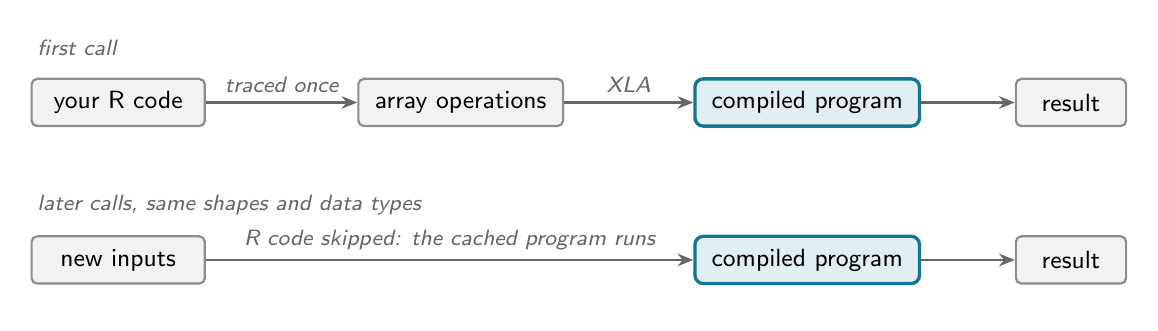
\begin{tikzpicture}
  \path[use as bounding box] (0, 0) rectangle (14, 3.5);
  \node[lbl, anchor=west] at (0, 3.25) {first call};
  \node[op, minimum width=2.2cm] (code) at (1.15, 2.55) {your R code};
  \node[op, minimum width=2.6cm] (ops) at (5.5, 2.55) {array operations};
  \node[ours, minimum width=2.6cm] (prog) at (9.9, 2.55) {compiled program};
  \node[op, minimum width=1.4cm] (out) at (13.25, 2.55) {result};
  \draw[arr] (code) -- node[above, lbl] {traced once} (ops);
  \draw[arr] (ops) -- node[above, lbl] {XLA} (prog);
  \draw[arr] (prog) -- (out);
  \node[lbl, anchor=west] at (0, 1.25) {later calls, same shapes and data types};
  \node[op, minimum width=2.2cm] (in2) at (1.15, 0.55) {new inputs};
  \node[ours, minimum width=2.6cm] (prog2) at (9.9, 0.55) {compiled program};
  \node[op, minimum width=1.4cm] (out2) at (13.25, 0.55) {result};
  \draw[arr] (in2) -- node[above, lbl] {R code skipped: the cached program runs} (prog2);
  \draw[arr] (prog2) -- (out2);
\end{tikzpicture}

% --- 2. the stack under {anvl} ---------------------------------------------------------
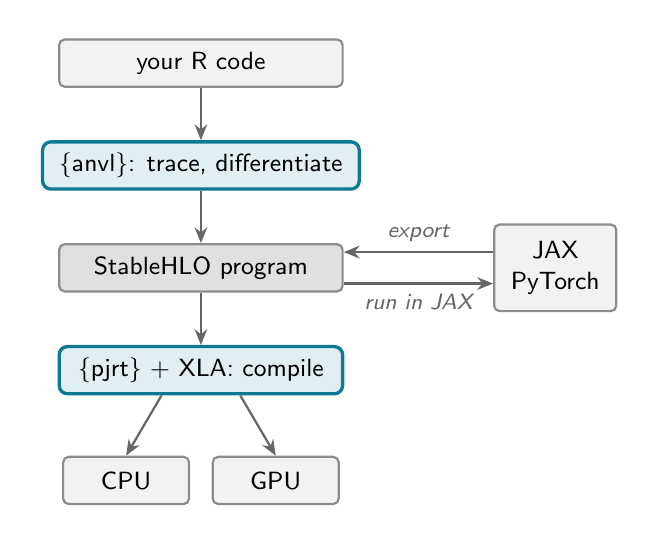
\begin{tikzpicture}
  \path[use as bounding box] (0, 0) rectangle (7.6, 6.2);
  \node[op, minimum width=3.6cm] (code) at (2.2, 5.75) {your R code};
  \node[ours, minimum width=3.6cm] (anvl) at (2.2, 4.45) {\{anvl\}: trace, differentiate};
  \node[op, minimum width=3.6cm, fill=black!12] (shlo) at (2.2, 3.15) {StableHLO program};
  \node[ours, minimum width=3.6cm] (pjrt) at (2.2, 1.85) {\{pjrt\} + XLA: compile};
  \node[op, minimum width=1.6cm] (cpu) at (1.25, 0.45) {CPU};
  \node[op, minimum width=1.6cm] (gpu) at (3.15, 0.45) {GPU};
  \node[op, minimum width=1.5cm, minimum height=1.1cm] (jax) at (6.7, 3.15) {JAX\\PyTorch};
  \draw[arr] (code) -- (anvl);
  \draw[arr] (anvl) -- (shlo);
  \draw[arr] (shlo) -- (pjrt);
  \draw[arr] (pjrt.south) ++(-0.5, 0) -- (cpu.north);
  \draw[arr] (pjrt.south) ++(0.5, 0) -- (gpu.north);
  % Programs come in from JAX and PyTorch, and {anvl} programs go out to JAX.
  \draw[arr] ($(jax.west) + (0, 0.2)$) -- node[above, lbl] {export} ($(shlo.east) + (0, 0.2)$);
  \draw[arr] ($(shlo.east) + (0, -0.2)$) -- node[below, lbl] {run in JAX} ($(jax.west) + (0, -0.2)$);
\end{tikzpicture}


% --- 3. and 4. column-major and row-major order -----------------------------------------
% The matrix is matrix(1:6, nrow = 2); the path visits its cells in memory order,
% and the strip below lists the values in that order.
\newcommand{\majororder}[2]{
  \begin{tikzpicture}
    \path[use as bounding box] (0, 0) rectangle (3.6, 3.0);
    \foreach \v/\x/\y in {1/1.2/2.35, 3/1.8/2.35, 5/2.4/2.35, 2/1.2/1.75, 4/1.8/1.75, 6/2.4/1.75}
      \coordinate (c\v) at (\x, \y);
    \draw[black!45, thick, fill=black!4] (0.9, 1.45) rectangle (2.7, 2.65);
    \draw[accent!70, line width=2.2pt, rounded corners=4pt, -{Stealth[length=2.6mm, width=2.4mm]}] #1;
    \foreach \v in {1, ..., 6}
      \node[circle, fill=white, inner sep=1.2pt, font=\ttfamily\small] at (c\v) {\v};
    \foreach \v [count=\i] in {#2}
      \node[draw=black!55, thick, fill=black!5, minimum size=0.48cm, inner sep=0pt,
        font=\ttfamily\small] at ({0.3 + 0.5 * \i}, 0.55) {\v};
    \node[font=\footnotesize\itshape, text=black!60] at (1.8, 1.05) {in memory};
  \end{tikzpicture}
}

\majororder{(c1) -- (c2) -- (c3) -- (c4) -- (c5) -- (c6)}{1, 2, 3, 4, 5, 6}
\majororder{(c1) -- (c3) -- (c5) -- (c2) -- (c4) -- (c6)}{1, 3, 5, 2, 4, 6}

% --- 5. gradient(): forward graph and backward pass -------------------------------------
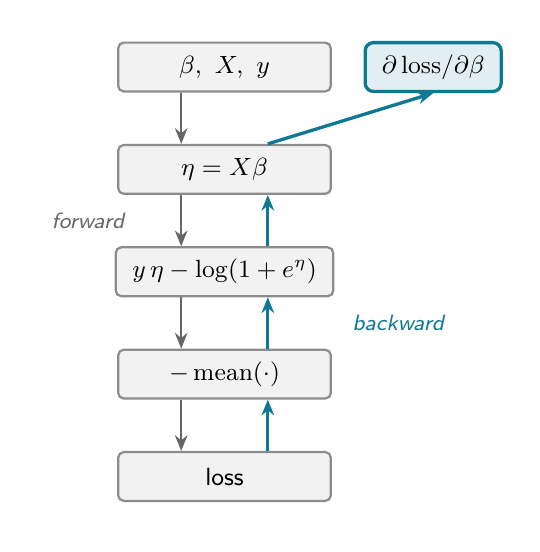
\begin{tikzpicture}
  \path[use as bounding box] (-0.75, 0) rectangle (5.4, 6.3);
  \tikzset{gnode/.style={op, minimum width=2.7cm, minimum height=0.62cm}}
  \node[gnode] (in) at (1.75, 5.8) {$\beta,\ X,\ y$};
  \node[gnode] (eta) at (1.75, 4.5) {$\eta = X\beta$};
  \node[gnode] (ll) at (1.75, 3.2) {$y\,\eta - \log(1 + e^{\eta})$};
  \node[gnode] (m) at (1.75, 1.9) {$-\,\mathrm{mean}(\cdot)$};
  \node[gnode] (loss) at (1.75, 0.6) {loss};
  \node[ours, minimum height=0.62cm] (grad) at (4.4, 5.8) {$\partial\,\mathrm{loss} / \partial\beta$};
  \foreach \a/\b in {in/eta, eta/ll, ll/m, m/loss}
    \draw[arr] ($(\a.south) + (-0.55, 0)$) -- ($(\b.north) + (-0.55, 0)$);
  \foreach \a/\b in {loss/m, m/ll, ll/eta}
    \draw[arr, draw=accent, very thick] ($(\a.north) + (0.55, 0)$) -- ($(\b.south) + (0.55, 0)$);
  \draw[arr, draw=accent, very thick] ($(eta.north) + (0.55, 0)$) -- (grad.south);
  \node[lbl, anchor=east] at (0.6, 3.85) {forward};
  \node[lbl, text=accent, anchor=west] at (3.25, 2.55) {backward};
\end{tikzpicture}

\end{document}
